\documentclass[letterpaper]{article}
\usepackage{graphicx}
\usepackage[left=3cm,top=2cm,bottom=2cm,right=3cm]{geometry}
\usepackage[title,titletoc]{appendix}
\usepackage{authblk}

\title{An Associative Memory-based Time-Multiplexed Pattern Recognition Engine for Track Trigger Systems
\\Fermilab Technical Memo TM-XXXX-X}

% % \author[3]{Sudha Ajuha}
% \author[3]{Andr\'{e} Cascadan}
% \author[3]{Thiago Costa de Paiva}
% \author[5]{Souvik Das}
% \author[6]{Ricardo Eusebi}
% \author[3]{Vitor Finotti Ferreira}
% \author[4]{Kristian Hahn}
% \author[1]{Zhen Hu}
\author[1]{Sergo Jindariani}
% \author[5]{Jacobo Konigsberg}
\author[1]{Tiehui Ted Liu}
% \author[5]{Jia Fu Low}
% \author[1]{Yasuyuki Okumura}
\author[1]{Jamieson Olsen}
% \author[3]{Lucas Arruda Ramalho}
% \author[5]{Roberto Rossin}
\author[1]{Luciano Ristori}
% \author[1]{Nhan Tran}
% \author[4]{Marco Trovato}
% \author[6]{Keith Ulmer}
% \author[3]{M\'{a}rio Vaz}
% \author[4]{Xianshan Wen}
% \author[1]{Jin-Yuan Wu}
% \author[1,2]{Zijun Xu}
% \author[4,7]{Silvia Zorzetti}

\affil[1]{Fermi National Accelerator Laboratory\footnote{Operated by Fermi Research Alliance, LLC under Contract No. DE-AC02-07CH11359 with the United States Department of Energy.}, Batavia, Illinois USA}
% \affil[2]{Peking University, Beijing CHINA}
% \affil[3]{UNESP - S\~{a}o Paulo State University, S\~{a}o Paulo BRAZIL}
% \affil[4]{Northwestern University, Evanston, Illinois USA}
% \affil[5]{University of Florida, Gainesville, Florida USA}
% \affil[6]{Texas A\&M University, College Station, Texas USA}
% \affil[7]{CERN, Geneva SWITZERLAND}

\date{\today}

% Alter some LaTeX defaults for better treatment of figures:
% See p.105 of "TeX Unbound" for suggested values.
% See pp. 199-200 of Lamport's "LaTeX" book for details.
%   General parameters, for ALL pages:
\renewcommand{\topfraction}{0.9}	% max fraction of floats at top
\renewcommand{\bottomfraction}{0.8}	% max fraction of floats at bottom
%   Parameters for TEXT pages (not float pages):
\setcounter{topnumber}{2}
\setcounter{bottomnumber}{2}
\setcounter{totalnumber}{4}     % 2 may work better
\setcounter{dbltopnumber}{2}    % for 2-column pages
\renewcommand{\dbltopfraction}{0.9}	% fit big float above 2-col. text
\renewcommand{\textfraction}{0.07}	% allow minimal text w. figs
%   Parameters for FLOAT pages (not text pages):
\renewcommand{\floatpagefraction}{0.7}	% require fuller float pages
% N.B.: floatpagefraction MUST be less than topfraction !!
\renewcommand{\dblfloatpagefraction}{0.7}	% require fuller float pages
% remember to use [htp] or [htpb] for placement



\begin{document}

\maketitle

% \begin{center}
% Operated by Fermi Research Alliance, LLC
% \\under Contract No. DE-AC02-07CH11359 
% \\with the United States Department of Energy.
% \end{center}

\begin{center}
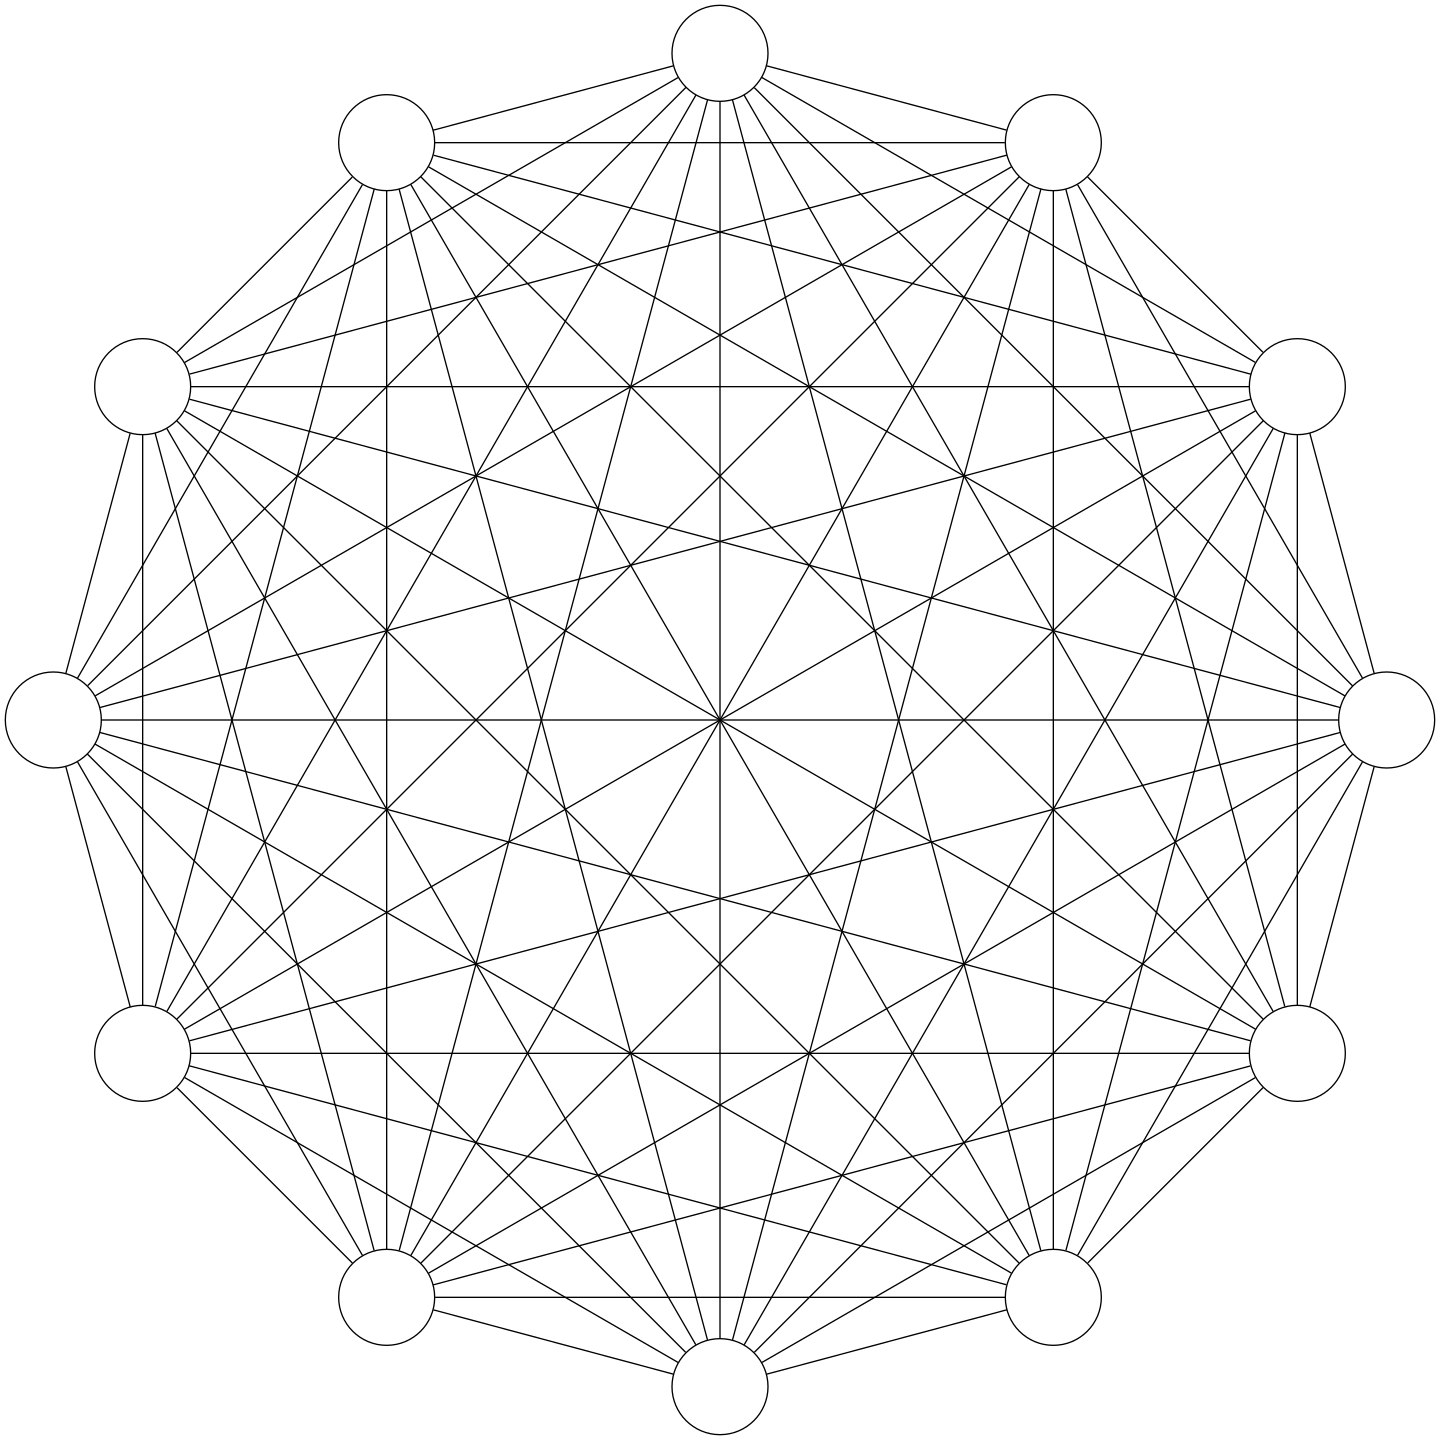
\includegraphics[width=4cm]{fullmesh.png}
\end{center}

\begin{abstract}
\noindent Pattern recognition associative memory (PRAM) devices are parallel processing engines which are used to tackle the complex combinatorics of track finding algorithms, particularly for silicon based tracking triggers. In this paper we present our latest PRAM-based track finder mezzanine card design which supports both ASIC and FPGA based PRAMs, and describe how the PRAM interface and FPGA firmware modules work in conjunction to implement a high performance fully pipelined low latency track finder and track fitter.  This work is part of the overall program for Level-1 silicon-based tracking trigger generic R\&D for high luminosity LHC.
\end{abstract}


\newpage
\tableofcontents
\listoffigures
\listoftables

\newpage

\section{Introduction}

\section{Demonstration System Design}

Before we launch into the demonstration system hardware details, it's worth documenting some of the basic assumptions that guided our design decisions. These choices are conservative, and were made up front so that the demonstration system hardware can be realized with technology available today. While the technology presented in this paper is certainly cutting edge it is not \emph{bleeding edge}. We aim to a practical system which uses ``modestly sized" FPGAs and is designed using conventional printed circuit board materials and layout techniques. At the conclusion of this paper we will discuss areas where performance improvements may be necessary, and how these improvements maybe realized through the use of faster, larger FPGAs, higher bandwidth connections, etc.

\subsection{System Assumptions}

\begin{itemize}

\item The accelerator bunch crossing (BX) frequency is 40MHz (25ns period).

\item The tracker sub-detector is subdivided into roughly symmetric and equal size trigger towers. Each tower consists of appoximately 320 silcon detector modules.

\item Data duplication and sharing across trigger tower boundaries is on the order of 10\%. Thus a trigger tower processor unit will need to import 32 modules from neighboring towers for a total of 352 inputs.

\item Silicon detector modules transmit the local coordinates of stubs (hit-pairs above a pT threshold) over a fiber optic link. The number of stubs reported per BX may vary. Derandomization is achiveved by packaging stubs for 8 consecutive BX into a fixed length ``train" or record of 200ns. Modules are synchronized to the beam and transmit these records continuously with no gaps in between.

\item Latency budget is 4$\mu$s as measured from the start of the input record to the first found track parameters on the output.

\end{itemize}

\subsection{Hardware Assumptions}

\begin{itemize}

\item A trigger tower processor consists of a single 14 slot ATCA shelf with 12 processor blades. The two hub slots are reserved for such items as commercially available Ethernet switch blades or custom blades used for DAQ readout, timing, etc.

\item An additional hardware layer positioned immediately upstream from the trigger tower processor shelf is responsible for data duplication and sharing across trigger tower boundaries. In this paper we present an architecture where there is no direct communication path between trigger tower processor shelves. (Note that the system architecture presented here is extremely flexible and is in fact capable of exchanging data between shelves, thereby eliminating the need for this additional upstream hardware layer. This alternate configuration will be presented in a separate paper.)

\item All 12 blades in the shelf receive input fibers from upstream hardware. An input fiber may be connected to any available input on any processor blade in the shelf. Our data distribution scheme insures that all incoming stubs are properly routed to the correct blade over the ATCA full mesh backplane.

\item All 12 processing blades in the shelf take part in data distribution, pattern recognition and track finding. Events are distributed amongst the 12 blades in a round robin fashion; thus the time multiplex factor is equal to 12 and each processing blade receives a new event every 300ns.

\item A Pattern Recognition Associative Memory (PRAM) device is used to in conjunction with an FPGA on the processor blade. The PRAM device may be implented as either an ASIC or FPGA. In this paper we consider the PRAM to be a black box: the PRAM interface is defined and the PRAM operation is described at a high level. Low level PRAM implementation details are covered in other documents.  

\item We choose to limit the serial transceiver line rates to 16Gbps for copper links. Supporting line rates above 16Gbps requires the use UltraScale Virtex parts in the more expensive mid-speed grades.  Likewise, we choose to limit fiber optic link speeds to 14Gbps as these optical devices are widely available, inexpensive commodity parts.

\item Serial transceivers will use conventional 8b/10b line encoding as it is natively supported in the FPGA transceiver and can be configured for the lowest achievable transmission latency.

\end{itemize}







\section{Hardware Design}

\subsection{Overview}

\begin{figure}
\centering
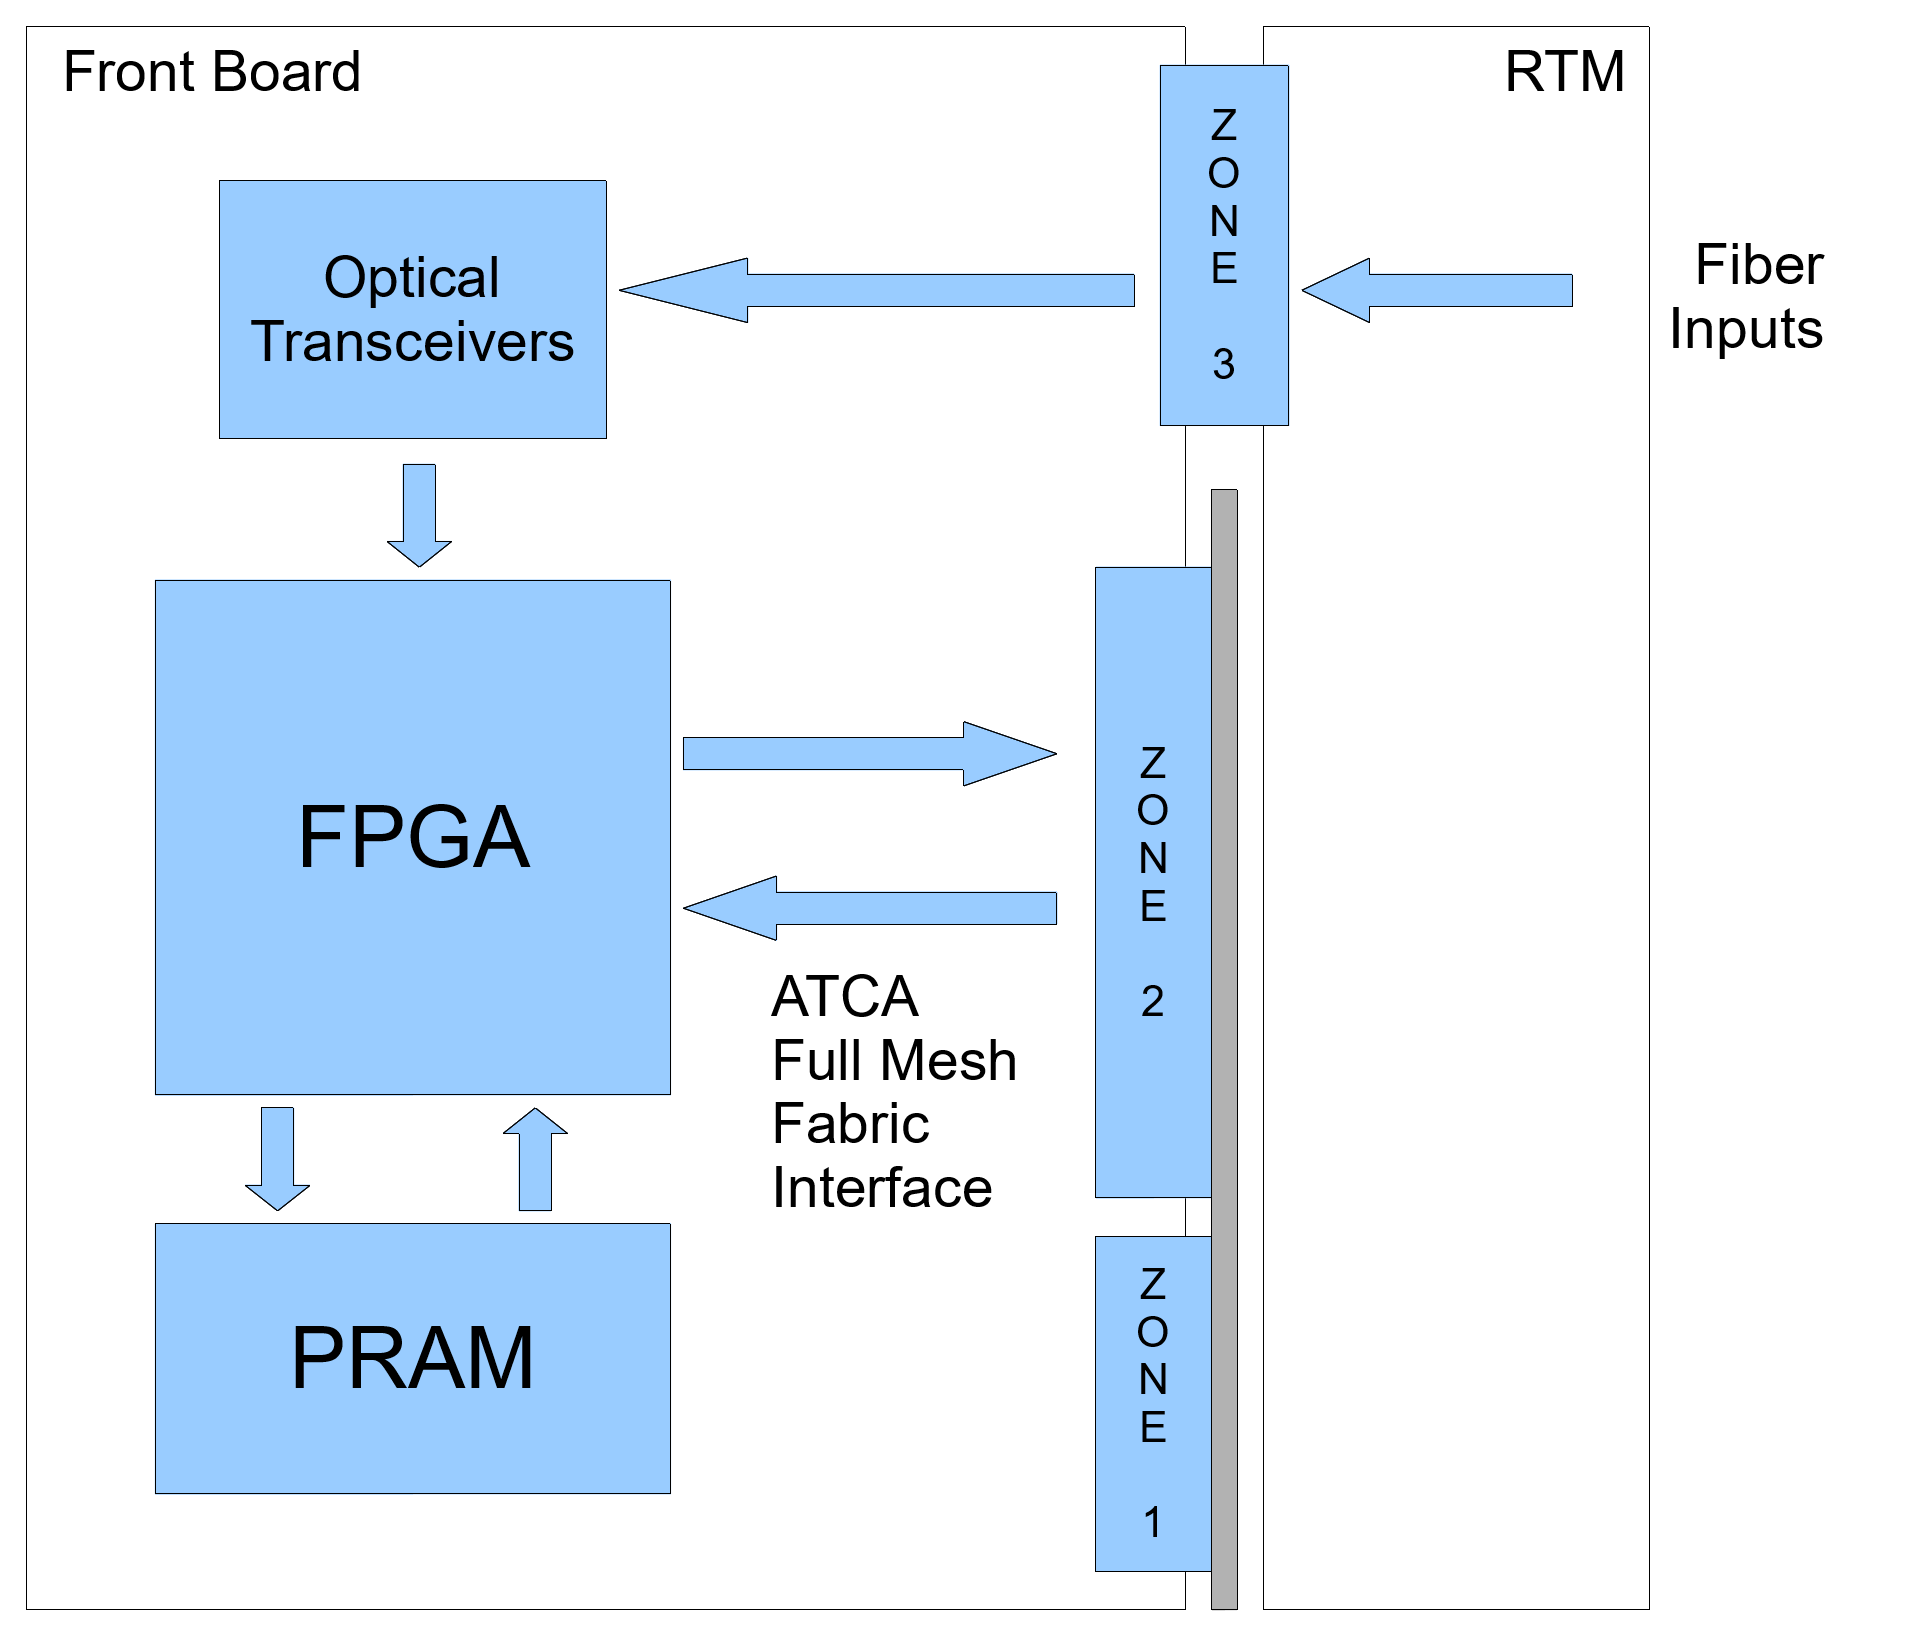
\includegraphics[width=16cm]{hwblock.png}
\caption{Processing board functional blocks.}
\label{hwblock}
\end{figure}

The hardware reference design consists of 12 processing boards installed in an ATCA shelf.  All processing boards use the full mesh fabric interface links to exchange data over the backplane.  The simplified block diagram for a processing board is shown in Figure \ref{hwblock}.  In this example reference design the Pattern Recognition Associative Memory (PRAM) functions are implemented in an ASIC (or, an FPGA where a subset of the ASIC is emulated).

\subsection{Pulsar3a Board}








\section{Firmware Design}

\subsection{Overview}

\begin{figure}
\centering
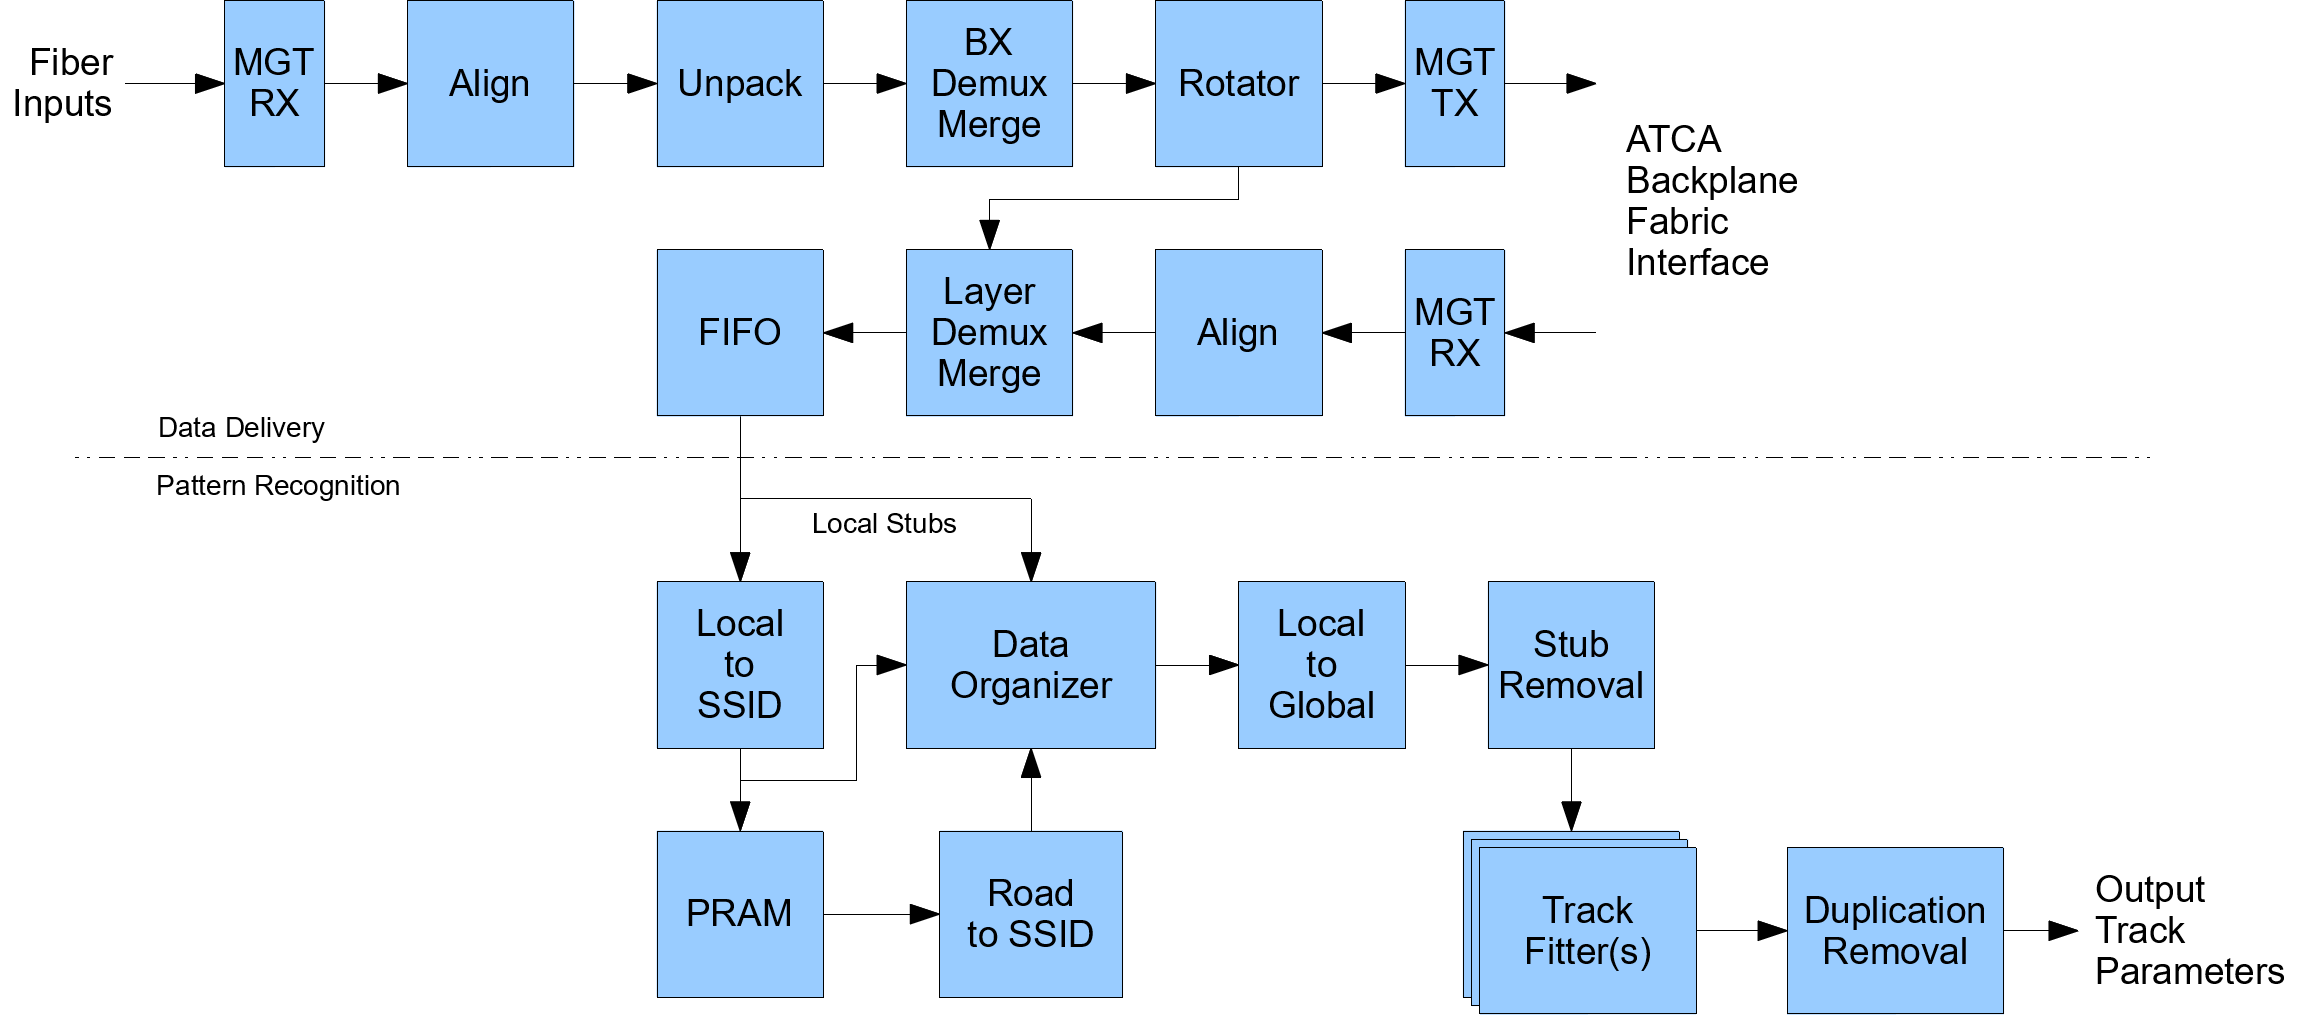
\includegraphics[width=16cm]{fwblock.png}
\caption{Firmware functional blocks.}
\label{fwblock}
\end{figure}

\subsection{Front-End Data Delivery}

\subsubsection{MGT RX}

Stubs arrive over multiple high speed fiber optic links from upstream modules.  Multi-gigabit transceivers (MGTs) in the FPGA receive this serial data, recover the clock, and convert the serial stream into 32-bit or 64-bit parallel words.  The serial encoding scheme defines various control sequences or markers which are used by the deserializer logic to determine word boundaries.

\subsubsection{Align}

Each fiber input link is in effect a unique clock domain.  It is assumed that all input links are frequency locked to the master accelerator clock; however no assumption can be made concerning the phase relationship between MGT recovered clocks.  The alignment block uses shallow FIFOs and control logic to transfer fiber input data from the various link clock domains into the FPGA master clock domain.  Typically the FPGA master clock runs at 240MHz to 400MHz and is frequency locked to the accelerator.  Dedicated signals on the ATCA backplane insure that all boards in the crate are synchronized to better than one BX.

\subsubsection{Unpack}

Stubs are densely packed into the input record format.  Furthermore, stubs do not align to 32-bit or 64-bit boundaries.  Internal buses in the FPGA are designed to transfer one stub per clock cycle, so for this reason, the entire input record must be stored in shift registers in the unpacker firmware block.

\subsubsection{BX Demux and Merge}

Stubs are sorted by BX and merged into 8 streams.  200ns.

\subsubsection{Rotator}

The Rotator block directs the eight stub streams to their destination board.  Each stub stream is directed to one of 12 possible destinations; 11 are in different boards and 1 is within the current processor board.  The demux assignments change every 200ns in order to effectively use all processing boards in the shelf.  This is where the time multiplexing occurs.  Eight out of 12 boards are always actively receiving stub data from the backplane.  Rotation figure.

\subsubsection{MGT TX and RX for Backplane Fabric}

Fabric Interface MGT transceivers serialize data transfers to neighboring processing boards in the shelf.  These transceivers are optimized for low latency transmission on the order of 150ns which is achieved by turning off and bypassing various elastic buffers and clock correction circuitry.

The Align Block uses shallow FIFOs are to cross from the MGT RX recovered clock domain back into the FPGA master clock domain.  Stubs which are not shared with any other processing boards in the shelf are delayed appropriately to line up with the streams from other boards in the shelf.

\subsubsection{Layer Demux and Merge}

At this point ALL stubs for a given BX received by a ALL processing boards in the shelf have been directed to this point.  Before stub data is directed to the PRAM it must be sorted by detector layer.  This module performs the demux and merge operation with minimal overhead as shown by the tree of sort nodes in Figure XXX.  Every 200ns a new event arrives.

\subsubsection{FIFO}

Thus far all firmware blocks are tied to the fiber input record rate; a new train/BX arrives every 200ns.  Time muliplexing with 12 processors allows for longer processing time and this FIFO is used to absorb the 200ns transmission ``bursts" and allows the remaining firmware modules to run continuously with a 300ns period.

\subsection{Pattern Recogition Associative Memory}

Six layers in, roads out.  This needs to be own section.  Separate chip with low latency LVDS parallel interface.  64k, 128k, 256k patterns defined.

\subsection{Backend Pattern Recogition Stage}

\subsubsection{Local to SSID}

BlockRAM based lookup tables and additional glue logic is used to determine the super-strip ID for the incoming local stubs.  Six blocks are required; one per layer.  Latency is a few clock cycles.  The SSID is 8 or 9 bits depending on detector layer.

\subsubsection{Data Organizer}

The Data Organizer is a type of database that enables local stubs to be stored in RAM at the address specified by the SSID.  Multiple local stubs may be stored at the same address without incurring any time penalty as read-modify-write cycles have been elimiated.  The DO is fully pipelined; as stubs for the current event are being stored, stubs for the previous event are being read out.

\subsubsection{Road to SSID}

Another lookup table function implented in BlockRAM.

\subsubsection{Local to Global}

Another lookup table function.  6 layers x 4 stubs per layer = up to 24 global stub streams.

\subsubsection{Stub Removal}

Knock down the combinatorics.  Worst case is 24 stubs or 4096 combinations to check.  Use Hough Transform and Luciano's algorithm to dramatically knock down the number of combinations.  Low latency and fully pipelined.

\subsubsection{Track Fitters}

Calculate given a set of 6 stubs (one per layer) this block calculates track parameters.  Fully pipelined and can accept a net set of stubs on each clock cycle.  Latency is about 50 clocks.  Based on simulation studies we believe that 7 Track Fitters in parallel should be sufficient.

\subsubsection{Duplication Removal}

N track fitters operating in parallel.  Choose the BEST result and pass along to downstream.

















\end{document}
